\documentclass[tikz]{standalone}
\usetikzlibrary{positioning, arrows.meta}
\begin{document}
    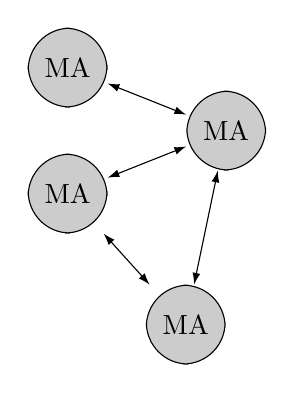
\begin{tikzpicture}[
        MA/.style = {draw, black, fill=black!20, minimum height=1cm, minimum width=1cm, rounded corners=15pt, inner sep=2pt},%
        arrow/.style = {{Latex[length=1.5mm, width=1.0mm]}-{Latex[length=1.5mm, width=1.0mm]},align=flush center}%
    ]%
        \node[MA] (1) {MA};
        \node[MA, right=1cm of 1, yshift=0.8cm] (2) {MA};
        \node[MA, left=1cm of 2, yshift=0.8cm] (3) {MA};
        \node[MA, below=2.25cm of 3, xshift=1.5cm] (4) {MA};
        \draw[arrow] (1) -> (2);
        \draw[arrow] (3) -> (2);
        \draw[arrow] (4) -> (2);
        \draw[arrow] (1) -> (4);
    \end{tikzpicture}
\end{document}